\chapter{Patrones De Diseño}
	\section{Qué Son Los Patrones De Diseño}
Los patrones de diseño son la base para la búsqueda de soluciones a problemas comunes en el desarrollo de software y
otros ámbitos referentes al diseño de interacción o interfaces. Un patrón describe un problema que ocurre varias
veces en un sistema, y la base de la solución a ese problema. Los patrones de diseño son el resultado del consenso de
los profesionales en el área y brindan herramientas a los diseñadores de sistemas para no escoger malos caminos,
valiéndose de documentación disponible en lugar de simplemente la intuición.

    \section{Patrones}
Un patrón de diseño es una solución a un problema de diseño. Para que una solución sea considerada un
patrón debe poseer ciertas características. Una de ellas es que se debe haber comprobado su efectividad resolviendo
problemas similares en ocasiones anteriores. Otra es que debe ser reusable, lo que significa que es aplicable a
diferentes problemas de diseño en distintas circunstancias. Cada patrón de diseño se focaliza sobre un problema o issue
particular de diseño (DOO).

En general, un patrón tiene cinco elementos esenciales:
        \begin{enumerate}
            \item \textbf{El nombre del patrón} nombre estándar del patrón por el cual será reconocido en la comunidad
(normalmente se expresan en inglés), se usa para describir un problema de diseño, su solución, y consecuencias.

            \item \textbf{Tipo} Clasificación en la que se encuentra el patrón, éstos pueden ser:
                \begin{itemize}
                    \item \textit{Creacionales}:Muestran la guía de cómo crear objetos cuando
sus creaciones requieren tomar decisiones. Estas decisiones normalmente serán resultas dinámicamente decidiendo que
clases instanciar o sobre que objetos un objeto delegará responsabilidades
                    \item \textit{Estructurales}: Describen la forma en que diferentes tipos de
objetos pueden ser organizados para trabajar unos con otros
                    \item \textit{Comportamiento}: Se utilizan para organizar, manejar y combinar comportamientos
                \end{itemize}

            \item \textbf{El problema} describe cuando aplicar el patrón, explica el problema y su contexto. También
                describe problemas de diseño específicos tales como ``Como representar un algoritmo como un objeto''.
                Además, describe la estructura de clases y objetos que son sintomáticas de un diseño inflexible. A
                veces, el problema puede incluir una lista de condiciones que deben ser reunidas antes de que tenga
                sentido aplicar el patrón. \item \textbf{La solución} describe los elementos que integran el
                diseño, sus relaciones, responsabilidades y colaboración. La solución no describe un diseño
                particular concreto o implementación, porque un patrón puede ser aplicado en muchas situaciones
                diferentes. De hecho, el patrón provee una descripción abstracta de un problema de diseño y
                como una disposición general de los elementos lo resuelve.
            \item \textbf{Las consecuencias} son los resultados y compromisos de aplicar el patrón. Estas son
                fundamentales para evaluar alternativas de diseño y para la comprensión de los costos y
                beneficios de aplicar el patrón. Las consecuencias de un patrón incluye su impacto sobre la
                flexibilidad del sistema, expansión o portabilidad.
        \end{enumerate}

	\section{Patrones Utilizados En \rc{}}
        A lo largo del proceso de diseño se encontraron problemas que coincidían con patrones. Estos patrones se
        explican brevemente a continuación:

        \subsection{Chain of Responsibility}\label{chain_pattern}
Proporcionar a más de un objeto la capacidad de atender una petición, para así evitar el acoplamiento con el que objeto
que hace la petición. Se forma con estos objetos una cadena, en la cual cada objeto o satisface la petición o la pasa al
siguiente.



    \subsubsection{Aplicabilidad}
        Este patrón es usado cuando:
        \begin{itemize}
            \item Hay más de un objeto que pueden manejar una petición, y el manejador no se conoce a priori, sino que
                debería determinarse automáticamente.
            \item Se quiere enviar una petición a un objeto entre varios sin especificar explícitamente el receptor.
            \item El conjunto d objetos que pueden tratar una petición debería ser especificado dinámicamente.
        \end{itemize}

    \subsubsection{Participantes}
        Entidades que forman parte del patrón.
        \begin{itemize}
            \item \textit{Client}: será el encargado de generar las peticiones que hayan de pasar por el manejador
                genérico.
            \item \textit{Handler}: deberá  estar  compuesto  por  un  interfaz  donde  se vayan a desarrollar las
                    peticiones que genera el cliente.
            \item \textit{Concrete Handler}: tratará  la  petición  que  le  corresponda del cliente según su criterio.
        \end{itemize}

    \subsubsection{Estructura}

    \begin{figure}[!h]
        \centering
        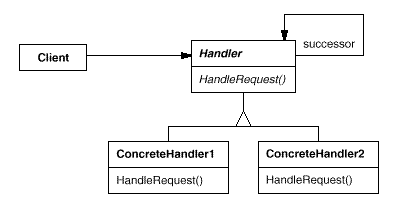
\includegraphics[scale=0.8]{images/chain-of-responsibility}
        \caption{Patrón \textit{``Chain of Responsibility''}.} \label{chain_pattern_img}
    \end{figure}